\subsection{x86: \RU{3 аргумента}\EN{3 arguments}}

\subsubsection{MSVC}

\RU{Компилируем при помощи MSVC 2010 Express, и в итоге получим:}
\EN{When we compile it with MSVC 2010 Express we get:}

\begin{lstlisting}
$SG3830	DB	'a=%d; b=%d; c=%d', 00H

...

	push	3
	push	2
	push	1
	push	OFFSET $SG3830
	call	_printf
	add	esp, 16					; 00000010H
\end{lstlisting}

\RU{Всё почти то же, за исключением того, что теперь видно, что аргументы для \printf заталкиваются в стек в обратном порядке: самый первый аргумент заталкивается последним.}
\EN{Almost the same, but now we can see the \printf arguments are pushed onto the stack in reverse order. The first argument is pushed last.}

\RU{Кстати, вспомним, что переменные типа \Tint в 32-битной системе, как известно, имеет ширину 32 бита, это 4 байта}
\EN{By the way, variables of \Tint type in 32-bit environment have 32-bit width, that is 4 bytes}.

\RU{Итак, у нас всего 4 аргумента. $4*4 = 16$~--- именно 16 байт занимают в стеке указатель на строку плюс ещё 3 числа типа \Tint.}
\EN{So, we have 4 arguments here. $4*4 = 16$~---they occupy exactly 16 bytes in the stack: a 32-bit pointer to a string and 3 numbers of type \Tint.}

\index{x86!\Instructions!ADD}
\index{x86!\Registers!ESP}
\index{cdecl}
\RU{Когда при помощи инструкции \TT{ADD ESP, X} корректируется \glslink{stack pointer}{указатель стека} \ESP 
после вызова какой-либо функции, зачастую можно сделать вывод о том, сколько аргументов 
у вызываемой функции было, разделив X на 4.}
\EN{When the \gls{stack pointer} (\ESP register) has changed back by the \TT{ADD ESP, X}
instruction after a function 
call, often, the number of function arguments could be deduced by simply dividing X by 4.}

\RU{Конечно, это относится только к cdecl-методу передачи аргументов через стек, 
и только для 32-битной среды.}
\EN{Of course, this is specific to the \IT{cdecl} calling convention, 
and only for 32-bit environment.}

\ifx\LITE\undefined
\RU{См. также в соответствующем разделе о способах передачи аргументов через стек}
\EN{See also the calling conventions section}~(\myref{sec:callingconventions}).
\fi

\RU{Иногда бывает так, что подряд идут несколько вызовов разных функций, 
но стек корректируется только один раз, после последнего вызова:}
\EN{In certain cases where several functions return right after one another, the compiler could merge multiple \TT{``ADD ESP, X''} instructions into one, after the last call:}

\begin{lstlisting}
push a1
push a2
call ...
...
push a1
call ...
...
push a1
push a2
push a3
call ...
add esp, 24
\end{lstlisting}

\ifdefined\IncludeOlly
\clearpage
\subsubsection{MSVC \AndENRU \olly}
\index{\olly}

\RU{Попробуем этот же пример в}\EN{Now let's try to load this example in} \olly.
\RU{Это один из наиболее популярных win32-отладчиков пользовательского режима}\EN{It is one of the most 
popular user-land win32 debuggers}.
\RU{Мы можем компилировать наш пример в}\EN{We can compile our example in} MSVC 2012 
\RU{с опцией}\EN{with} \TT{/MD} \RU{что означает линковать с библиотекой}\EN{option, which means to link 
with} \TT{MSVCR*.DLL},
\RU{чтобы импортируемые функции были хорошо видны в отладчике.}
\EN{so we can see the imported functions clearly in the debugger.}

\RU{Затем загружаем исполняемый файл в}\EN{Then load the executable in} \olly.
\RU{Самая первая точка останова в}\EN{The very first breakpoint is in} \TT{ntdll.dll}, \RU{нажмите}\EN{press} 
F9 (\RU{запустить}\EN{run}).
\RU{Вторая точка останова в}\EN{The second breakpoint is in} \ac{CRT}-\RU{коде}\EN{code}.
\RU{Теперь мы должны найти функцию}\EN{Now we have to find the} \main\EN{ function}.

\RU{Найдите этот код прокрутив окно кода до самого верха (MSVC располагает функцию \main в самом начале
секции кода)}\EN{Find this code by scrolling the code to the very top (MSVC allocates the \main function at
the very beginning of the code section)}: 

\begin{figure}[H]
\centering
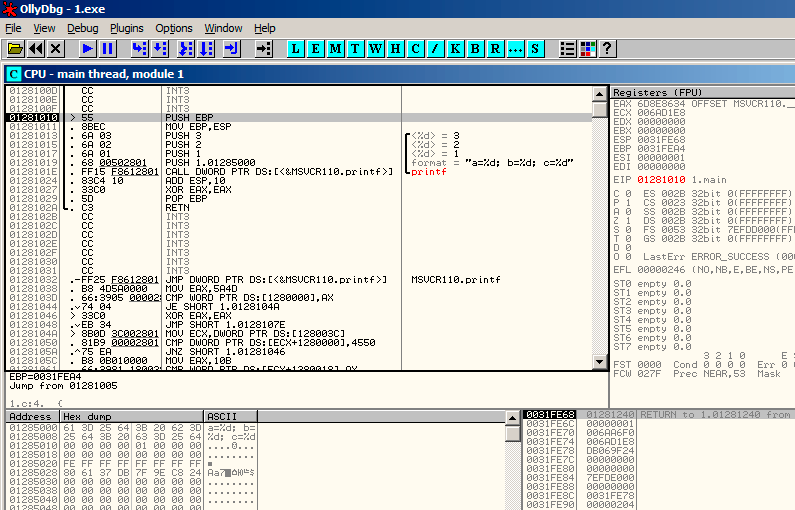
\includegraphics[scale=\FigScale]{patterns/03_printf/x86/olly3_1.png}
\caption{\olly: \RU{самое начало функции}\EN{the very start of the} \main\EN{ function}}
\label{fig:printf3_olly_1}
\end{figure}

\RU{Кликните на инструкции}\EN{Click on the} \TT{PUSH EBP}\RU{, нажмите}\EN{ instruction, press} F2 
(\RU{установка точки останова}\EN{set breakpoint}) \RU{и нажмите}\EN{and press} F9 (\RU{запустить}\EN{run}).
\RU{Нам нужно произвести все эти манипуляции, чтобы пропустить \ac{CRT}-код, потому что нам он пока
не интересен}\EN{We need to perform these actions in order to skip \ac{CRT}-code, because we aren't really
interested in it yet}.

\clearpage
\RU{Нажмите}\EN{Press} F8 (\stepover) 6 \RU{раз, т.е., пропустить
6 инструкций}\EN{times, i.e., skip 6 instructions}:

\begin{figure}[H]
\centering
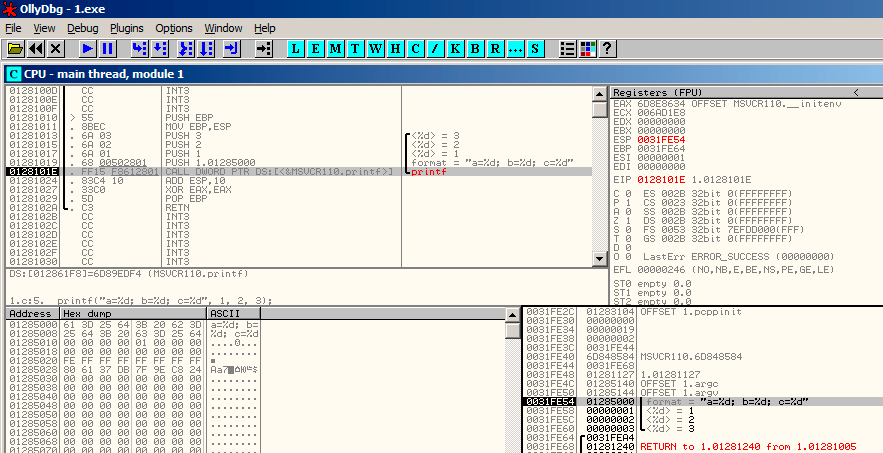
\includegraphics[scale=\FigScale]{patterns/03_printf/x86/olly3_2.png}
\caption{\olly: \RU{перед исполнением}\EN{before} \printf\EN{ execution}}
\label{fig:printf3_olly_2}
\end{figure}

\RU{Теперь}\EN{Now the} \ac{PC} \RU{указывает на инструкцию}\EN{points to the}
\TT{CALL printf}\EN{ instruction}.
\olly, \RU{как и другие отладчики, подсвечивает регистры со значениями, которые изменились}
\EN{like other debuggers, highlights the value of the registers which were changed}.
\RU{Поэтому каждый раз когда мы нажимаем}\EN{So each time you press} F8, \EIP 
\RU{изменяется и его значение подсвечивается красным}\EN{ changes and its value is displayed in red}.
\ESP \RU{также меняется, потому что значения заталкиваются в стек}\EN{changes as well, 
because the arguments values are pushed into the stack}.\\
\\
\RU{Где находятся эти значения в стеке}\EN{Where are the values in the stack}?
\RU{Посмотрите на правое нижнее окно в отладчике}\EN{Take a look at the right/bottom debugger window}:

\begin{figure}[H]
\centering
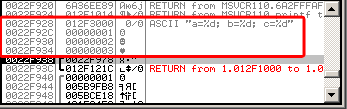
\includegraphics[scale=\NormalScale]{patterns/03_printf/x86/olly3_stack.png}
\caption{\olly: \RU{стек с сохраненными значениями}\EN{stack after the argument values have been pushed}
(\RU{красная рамка добавлена в графическом редакторе}\EN{The red rectangular border was added by me in a graphics editor})}
\end{figure}

\RU{Здесь видно 3 столбца: адрес в стеке, значение в стеке и ещё дополнительный комментарий
от \olly}\EN{We can see 3 columns there: address in the stack, 
value in the stack and some additional \olly comments}. 
\olly \RU{понимает}\EN{understands} \printf\RU{-строки}\EN{-like strings}, 
\RU{так что он показывает здесь и строку и 3 значения \IT{привязанных} к ней}\EN{so it reports the 
string here and the 3 values \IT{attached} to it}.

\RU{Можно кликнуть правой кнопкой мыши на строке формата, кликнуть на ``Follow in dump''
и строка формата появится в окне слева внизу, где всегда виден какой-либо участок памяти}%
\EN{It is possible to right-click on the format string, click on ``Follow in dump'',
and the format string will appear in the debugger left-bottom window, which always displays some part of the memory}.
\RU{Эти значения в памяти можно редактировать}\EN{These memory values can be edited}.
\RU{Можно изменить саму строку формата, и тогда результат работы нашего примера будет другой}%
\EN{It is possible to change the format string, in which case the result of our example would be different}.
\RU{В данном случае пользы от этого немного, но для упражнения это полезно,
чтобы начать чувствовать как тут всё работает}\EN{It is not very useful in this particular case, but it could be good as an exercise so you start building a feel of how everything works here}.

\clearpage
\RU{Нажмите}\EN{Press} F8 (\stepover).

\RU{В консоли мы видим вывод}\EN{We see the following output in the console}:

\begin{figure}[H]
\centering
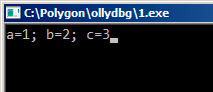
\includegraphics[scale=\NormalScale]{patterns/03_printf/x86/olly3_console.png}
\caption{\RU{Функция }\printf \RU{исполнилась}\EN{function executed}}
\end{figure}

\RU{Посмотрим как изменились регистры и состояние стека}\EN{Let's see how the registers and stack state 
have changed}: 

\begin{figure}[H]
\centering
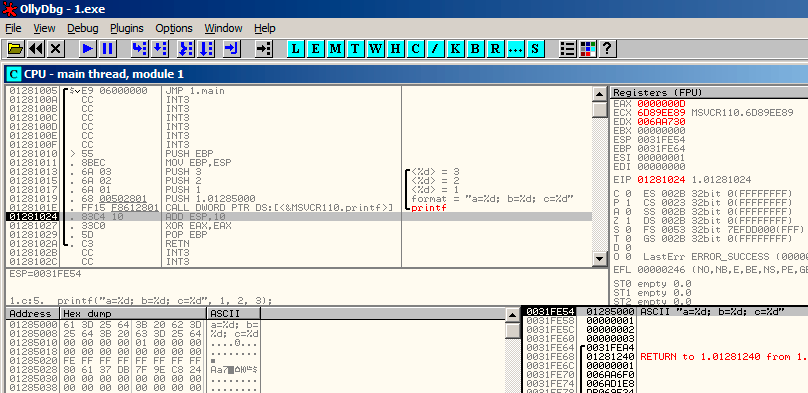
\includegraphics[scale=\FigScale]{patterns/03_printf/x86/olly3_3.png}
\caption{\olly \RU{после исполнения}\EN{after} \printf\EN{ execution}}
\label{fig:printf3_olly_3}
\end{figure}

\RU{Регистр }\EN{Register }\EAX \RU{теперь содержит}\EN{now contains} \TT{0xD} (13).
\RU{Всё верно: \printf возвращает количество выведенных символов.
Значение \EIP изменилось. Действительно, теперь здесь адрес инструкции после 
\TT{CALL printf}.}
\EN{That is correct, since \printf returns the number of characters printed. 
The value of \EIP has changed: indeed, now it contains the address of the instruction coming after 
\TT{CALL printf}.}
\RU{Значения регистров }\ECX \AndENRU \EDX \RU{также изменились}\EN{values have changed as well}.
\RU{Очевидно, внутренности функции \printf используют их для каких-то своих нужд}\EN{Apparently, the 
\printf function's hidden machinery used them for its own needs}.

\RU{Очень важно то, что значение \ESP не изменилось. И аргументы-значения в стеке также!}
\EN{A very important fact is that neither the \ESP value, nor the stack state have been changed!}
\RU{Мы ясно видим здесь и строку формата и соответствующие ей 3 значения, они всё ещё здесь.}
\EN{We clearly see that the format string and corresponding 3 values are still there.}
\RU{Действительно, по соглашению вызовов \IT{cdecl}, вызываемая функция не возвращает \ESP назад.}
\EN{This is indeed the \IT{cdecl} calling convention behaviour: \gls{callee} does not return \ESP back to its previous value.}
\RU{Это должна делать вызывающая функция}\EN{The \gls{caller} is responsible to do so}.

\clearpage
\RU{Нажмите}\EN{Press} F8 \RU{снова, чтобы исполнилась инструкция}\EN{again to execute} 
\TT{ADD ESP, 10}\EN{ instruction}:

\begin{figure}[H]
\centering
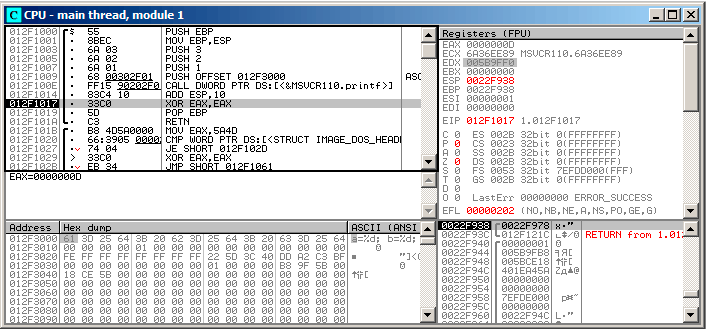
\includegraphics[scale=\FigScale]{patterns/03_printf/x86/olly3_4.png}
\caption{\olly: \RU{после исполнения инструкции}\EN{after} \TT{ADD ESP, 10}\EN{ instruction execution}}
\label{fig:printf3_olly_4}
\end{figure}

\ESP \RU{изменился, но значения всё ещё в стеке}\EN{has changed, but the values are still in the stack}!
\RU{Конечно, никому не нужно заполнять эти значения нулями или что-то в этом роде.}\EN{Yes, 
of course; no one needs to set these values to zeroes or something like that.}
\RU{Всё что выше указателя стека}\EN{Everything above the stack pointer} (\ac{SP}) 
\RU{это}\EN{is} \IT{\RU{шум}\EN{noise}} \OrENRU \IT{\garbage{}} \RU{и не имеет
особой ценности}\EN{and has no meaning at all}.
\RU{Было бы очень затратно по времени очищать ненужные элементы стека, к тому же, никому это и не 
нужно}\EN{It would be time consuming to clear the unused stack entries anyway, and no one really needs to}.

\fi

\ifdefined\IncludeGCC
\subsubsection{GCC}

\RU{Скомпилируем то же самое в Linux при помощи GCC 4.4.1 и посмотрим на результат в \IDA:}
\EN{Now let's compile the same program in Linux using GCC 4.4.1 and take a look at what we have got in \IDA:}

\begin{lstlisting}
main            proc near

var_10          = dword ptr -10h
var_C           = dword ptr -0Ch
var_8           = dword ptr -8
var_4           = dword ptr -4

                push    ebp
                mov     ebp, esp
                and     esp, 0FFFFFFF0h
                sub     esp, 10h
                mov     eax, offset aADBDCD ; "a=%d; b=%d; c=%d"
                mov     [esp+10h+var_4], 3
                mov     [esp+10h+var_8], 2
                mov     [esp+10h+var_C], 1
                mov     [esp+10h+var_10], eax
                call    _printf
                mov     eax, 0
                leave
                retn
main            endp
\end{lstlisting}

\RU{Можно сказать что этот короткий код, созданный GCC, отличается от кода MSVC только способом помещения 
значений в стек.
Здесь GCC снова работает со стеком напрямую без \PUSH/\POP.}
\EN{Its noticeable that the difference between the MSVC code and the GCC code is only in the way the arguments are stored on the stack.
Here the GCC is working directly with the stack without the use of \PUSH/\POP.}

\ifdefined\IncludeGDB
\subsubsection{GCC \AndENRU GDB}
\index{GDB}

\RU{Попробуем также этот пример и в \ac{GDB} в Linux}\EN{Let's try this example also in \ac{GDB} in Linux}.

\TT{-g} \RU{означает генерировать отладочную информацию в выходном исполняемом файле}\EN{option instructs the compiler to include debug information in the executable file}.

\begin{lstlisting}
$ gcc 1.c -g -o 1
\end{lstlisting}

\begin{lstlisting}
$ gdb 1
GNU gdb (GDB) 7.6.1-ubuntu
Copyright (C) 2013 Free Software Foundation, Inc.
License GPLv3+: GNU GPL version 3 or later <http://gnu.org/licenses/gpl.html>
This is free software: you are free to change and redistribute it.
There is NO WARRANTY, to the extent permitted by law.  Type "show copying"
and "show warranty" for details.
This GDB was configured as "i686-linux-gnu".
For bug reporting instructions, please see:
<http://www.gnu.org/software/gdb/bugs/>...
Reading symbols from /home/dennis/polygon/1...done.
\end{lstlisting}

\begin{lstlisting}[caption=\RU{установим точку останова на}\EN{let's set breakpoint on} \printf]
(gdb) b printf
Breakpoint 1 at 0x80482f0
\end{lstlisting}

\RU{Запукаем}\EN{Run}.
\RU{У нас нет исходного кода функции}\EN{We don't have the} \printf%
\RU{, поэтому \ac{GDB} не может его показать}\EN{function source code here, 
so \ac{GDB} can't show it, but may do so}.

\begin{lstlisting}
(gdb) run
Starting program: /home/dennis/polygon/1 

Breakpoint 1, __printf (format=0x80484f0 "a=%d; b=%d; c=%d") at printf.c:29
29	printf.c: No such file or directory.
\end{lstlisting}

\RU{Выдать 10 элементов стека. Левый столбец~--- это адрес в стеке.}
\EN{Print 10 stack elements. The most left column contains addresses on the stack.}

\begin{lstlisting}
(gdb) x/10w $esp
0xbffff11c:	0x0804844a	0x080484f0	0x00000001	0x00000002
0xbffff12c:	0x00000003	0x08048460	0x00000000	0x00000000
0xbffff13c:	0xb7e29905	0x00000001
\end{lstlisting}

\RU{Самый первый элемент это}\EN{The very first element is the} \ac{RA} (\TT{0x0804844a}).
\RU{Мы можем удостовериться в этом, дизассемблируя память по этому адресу}\EN{We can verify this by disassembling the memory at this address}:

\begin{lstlisting}
(gdb) x/5i 0x0804844a
   0x804844a <main+45>:	mov    $0x0,%eax
   0x804844f <main+50>:	leave  
   0x8048450 <main+51>:	ret    
   0x8048451:	xchg   %ax,%ax
   0x8048453:	xchg   %ax,%ax
\end{lstlisting}

\RU{Две инструкции}\EN{The two} \TT{XCHG} 
\RU{это, вероятно, какой-то случайный мусор, который мы пока что можем игнорировать}%
\EN{instructions are probably random garbage, which we can ignore for now}.

\RU{Второй элемент}\EN{The second element} (\TT{0x080484f0}) \RU{это адрес
строки формата}\EN{is the format string address}:

\begin{lstlisting}
(gdb) x/s 0x080484f0
0x80484f0:	"a=%d; b=%d; c=%d"
\end{lstlisting}

\RU{Остальные 3 элемента}\EN{Next 3 elements} (1, 2, 3) \RU{это аргументы функции}\EN{are the} 
\printf\EN{ arguments}.
\RU{Остальные элементы это может быть и мусор в стеке, но могут быть и значения
от других функций, их локальные переменные, и~т.д.}
\EN{The rest of the elements could be just ``garbage'' on the stack,
but could also be values from other functions, their local variables, etc.}
\RU{Пока что мы можем игнорировать их}\EN{We can ignore them for now}.

\RU{Исполняем}\EN{Run} ``finish''. 
\RU{Это значит исполнять все инструкции до самого конца функции}\EN{The command instructs GDB to ``execute all instructions until the end of the function''}. 
\RU{В данном случае это означает исполнять до завершения}\EN{In this case: execute till the end of} \printf.

\begin{lstlisting}
(gdb) finish
Run till exit from #0  __printf (format=0x80484f0 "a=%d; b=%d; c=%d") at printf.c:29
main () at 1.c:6
6		return 0;
Value returned is $2 = 13
\end{lstlisting}

\ac{GDB} \RU{показывает, что вернула}\EN{shows what} \printf \RU{в}\EN{returned in} \EAX (13).
\RU{Это, так же как и в примере с \olly, количество напечатанных символов}%
\EN{This is the number of characters printed out, just like in the \olly example}.

\RU{А ещё мы видим}\EN{We also see} ``return 0;'' \RU{и что это выражение находится в файле 
\TT{1.c} в строке 6}\EN{and the information that this expression is in the \TT{1.c} file at the line 6}.
\RU{Действительно, файл \TT{1.c} лежит в текущем директории и \ac{GDB} находит там эту строку}
\EN{Indeed, the \TT{1.c} file is located in the current directory, and \ac{GDB} finds the string there}.
\RU{Как \ac{GDB} знает, какая строка Си-кода сейчас исполняется}\EN{How does \ac{GDB} know which C-code line
is being currently executed}?
\RU{Компилятор, генерируя отладочную информацию,
также сохраняет информацию о 
соответствии строк в исходном коде и адресов инструкций}\EN{This is due to the fact that the compiler,
while generating debugging information, also saves a table of relations between source code line
numbers and instruction addresses}.
GDB \RU{это всё-таки отладчик уровня исходных текстов}\EN{is a source-level debugger, after all}.

\RU{Посмотрим регистры}\EN{Let's examine the registers}.
13 \InENRU \EAX:

\begin{lstlisting}
(gdb) info registers
eax            0xd	13
ecx            0x0	0
edx            0x0	0
ebx            0xb7fc0000	-1208221696
esp            0xbffff120	0xbffff120
ebp            0xbffff138	0xbffff138
esi            0x0	0
edi            0x0	0
eip            0x804844a	0x804844a <main+45>
...
\end{lstlisting}

\RU{Попробуем дизассемблировать текущие инструкции}\EN{Let's disassemble the current instructions}.
\RU{Стрелка указывает на инструкцию, которая будет исполнена следующей}\EN{The arrow points to the 
instruction to be executed next}.

\begin{lstlisting}
(gdb) disas
Dump of assembler code for function main:
   0x0804841d <+0>:	push   %ebp
   0x0804841e <+1>:	mov    %esp,%ebp
   0x08048420 <+3>:	and    $0xfffffff0,%esp
   0x08048423 <+6>:	sub    $0x10,%esp
   0x08048426 <+9>:	movl   $0x3,0xc(%esp)
   0x0804842e <+17>:	movl   $0x2,0x8(%esp)
   0x08048436 <+25>:	movl   $0x1,0x4(%esp)
   0x0804843e <+33>:	movl   $0x80484f0,(%esp)
   0x08048445 <+40>:	call   0x80482f0 <printf@plt>
=> 0x0804844a <+45>:	mov    $0x0,%eax
   0x0804844f <+50>:	leave  
   0x08048450 <+51>:	ret    
End of assembler dump.
\end{lstlisting}

\RU{По умолчанию} \ac{GDB} \RU{показывает дизассемблированный листинг в формате}\EN{uses} AT\&T 
\EN{syntax by default}.
\RU{Но можно также переключиться в формат Intel}\EN{It is possible to switch to Intel syntax}:

\begin{lstlisting}
(gdb) set disassembly-flavor intel
(gdb) disas
Dump of assembler code for function main:
   0x0804841d <+0>:	push   ebp
   0x0804841e <+1>:	mov    ebp,esp
   0x08048420 <+3>:	and    esp,0xfffffff0
   0x08048423 <+6>:	sub    esp,0x10
   0x08048426 <+9>:	mov    DWORD PTR [esp+0xc],0x3
   0x0804842e <+17>:	mov    DWORD PTR [esp+0x8],0x2
   0x08048436 <+25>:	mov    DWORD PTR [esp+0x4],0x1
   0x0804843e <+33>:	mov    DWORD PTR [esp],0x80484f0
   0x08048445 <+40>:	call   0x80482f0 <printf@plt>
=> 0x0804844a <+45>:	mov    eax,0x0
   0x0804844f <+50>:	leave  
   0x08048450 <+51>:	ret    
End of assembler dump.
\end{lstlisting}

\RU{Исполняем следующую инструкцию}\EN{Execute next instruction}.
\ac{GDB} \RU{покажет закрывающую скобку, означая, что это конец блока в функции}\EN{shows ending bracket, 
meaning, this ends the block}.

\begin{lstlisting}
(gdb) step
7	};
\end{lstlisting}

\RU{Посмотрим регистры после исполнения инструкции}\EN{Let's examine the registers after the} 
\TT{MOV EAX, 0}\EN{ instruction execution}. \EN{Indeed}
\EAX \RU{здесь уже действительно ноль}\EN{is zero at that point}.

\begin{lstlisting}
(gdb) info registers
eax            0x0	0
ecx            0x0	0
edx            0x0	0
ebx            0xb7fc0000	-1208221696
esp            0xbffff120	0xbffff120
ebp            0xbffff138	0xbffff138
esi            0x0	0
edi            0x0	0
eip            0x804844f	0x804844f <main+50>
...
\end{lstlisting}
\fi
\fi
